
\documentclass[11pt]{book}
%\documentclass[a4paper,twoside,11pt]{article}
%\documentclass[11pt]{article}

% \documentclass[a4paper,twoside]{report}

\usepackage[utf8]{inputenc}

%\documentclass[11pt]{adfathesis}
%\documentclass[11pt]{afthesis}
%\documentclass[11pt]{ebsthesis}
%\documentclass[11pt]{elteikthesis}
%\documentclass[11pt]{fbithesis}
%\documentclass[11pt]{gatech-thesis}
%\documentclass[11pt]{hepthesis}
%\documentclass[11pt]{kdgdocs}
%\documentclass[11pt]{msu-thesis}
%%\documentclass[11pt]{muthesis}
%\documentclass[11pt]{ryethesis}
%\documentclass[11pt]{sapthesis}
%\documentclass[11pt]{seuthesis}
%%\documentclass[11pt]{usthesis}
%\documentclass[11pt]{thuthesis}
%\documentclass[11pt]{my-thesis}
%\documentclass[11pt]{ua-thesis}
%\documentclass[11pt]{uafthesis}
%\documentclass[11pt]{ucdavisthesis}
%\documentclass[11pt]{ucthesis}
%\documentclass[11pt]{uiucthesis}
%\documentclass[11pt]{umich-thesis}
%\documentclass[11pt]{umthesis}
%\documentclass[11pt]{uothesis}
%\documentclass[11pt]{uowthesis}
%\documentclass[11pt]{ut-thesis}
%\documentclass[11pt]{uwthesis}
%\documentclass[11pt]{york-thesis}

\usepackage{epsfig}
\usepackage{graphicx}
\usepackage{algorithm}
\usepackage{algorithmic}
%\usepackage{algorithmic2}
\usepackage{verbatim}
\usepackage{multirow}
\usepackage[table]{xcolor}
\usepackage{color,colortbl}
\usepackage{url}
\usepackage{array}
\usepackage[bookmarks=true, pdftitle={Energy aware scheduling in heterogeneous computing systems}, pdfauthor={Gabriel Centurion}, colorlinks=true, linkcolor=black, citecolor=black, urlcolor=black]{hyperref}
\usepackage{bookmark}
\usepackage[spanish]{babel}
\usepackage{amssymb}
\usepackage{amsmath}
\usepackage{amsthm}
%\usepackage[fleqn]{amsmath}
\usepackage{ifthen}
% \usepackage{fancyhdr}
\usepackage{setspace}
\usepackage[section]{placeins}
%\usepackage[round,sort&compress]{natbib}
%\usepackage[round,compress]{natbib}
%\usepackage{subfigure}
\usepackage{caption}
\usepackage{subcaption}
\usepackage{rotating}
\usepackage{xfrac}
%\usepackage[titletoc]{appendix}
\usepackage{appendix}
\usepackage{bibentry}


%\theoremstyle{plain}
\theoremstyle{definition}
\newtheorem{mydef}{Definition}
%\definecolor{Gray}{gray}{0.9}

%\hoffset = -1in
\voffset = -1in
\topmargin = 30pt
\textheight = 650pt
\textwidth = 420pt
%\marginparwidth = 0pt
%\marginparsep = 0pt
\oddsidemargin = 0pt
\evensidemargin = 0pt



\begin{document}

% tells bibentry to (re)use the bibliographic data from the standard BibTeX setup
%\nobibliography*

% -- title page --
\pagenumbering{roman}
\begin{titlepage}
  \thispagestyle{empty}
  %\addtolength{\oddsidemargin}{0.5cm}
  \begin{center}
    %~\\[1.2cm]
    ~\\[0.0cm]
    \textsc{\Huge CECAL} \\[1.0cm]
    \textsc{\large Instituto de Computaci\'on, Facultad de Ingenier\'ia} \\[0.5cm]
    \textsc{\large Universidad de la Rep\'ublica} \\[0.2cm]
    \textsc{\large Montevideo, Uruguay} \\[2.5cm]
    \textsc{\Huge INFORME} \\[0.2cm]
    \textsc{\Huge PROYECTO DE GRADO} \\[2.0cm]
    \textbf{\huge Estudio experimental de frameworks } \\[0.2cm]
    \textbf{\huge para el desarrollo de Microservicios } \\[0.2cm]
    \textbf{\huge basado en el paradigma de computación } \\[0.2cm]
    \textbf{\huge distribuida} \\[2.5cm]
    {\Large Gabriel Centuri\'on} \\[0.2cm]
    {\Large gabriel.centurion@fing.edu.uy} \\[1.5cm]
    {\Large julio de 2022} \\[1.5cm]
    {\Large Tutor de Proyecto: \\[0.5cm] Sergio Nesmachnow, Universidad de la Rep\'ublica.} \\[1.0cm]
    
  \end{center}
  \vfill
\end{titlepage}
{
  \thispagestyle{empty}
  %\addtolength{\evensidemargin}{-1.5cm}
  ~\\[16cm]
  Estudio experimental de frameworks para el desarrollo de Microservicios \\[0.05cm]
  Centuri\'on, Gabriel \\[0.05cm]
  %ISSN 0797-6410 \\[0.05cm]
  Informe Proyecto de Grado \\[0.05cm]
  %Reporte T\'ecnico RT ??-?? \\[0.05cm]
  %PEDECIBA \\[0.05cm]
  Instituto de Computaci\'on - Facultad de Ingenier\'ia \\[0.05cm]
  Universidad de la Rep\'ublica \\[0.05cm]
  Montevideo, Uruguay, julio de 2022 \\[0.05cm]
  \vfill
  \cleardoublepage
}
\setcounter{page}{1}
\cleardoublepage

% \begin{abstract}


{
    \thispagestyle{empty}
    
    \begin{center}
    ~\\[0.2cm]
        \textsc{\huge Estudio experimental de frameworks para el desarrollo de Microservicios } \\[0.2cm] 
        \textsc{\huge basado en el paradigma de computación distribuida} \\[1cm]
        \textsc{\Large Abstract}
    \end{center}
    ~\\[0.2cm]
    \textbf{\large 
    Lorem ipsum dolor
    }
	~\\[1.0cm]
    \textbf{\large Keywords: Sed, euismod, turpis, ut, turpis}
}
\clearpage
{
    \begin{center}
     ~\\[0.2cm]
        \textsc{\huge Estudio experimental de frameworks } \\[0.2cm]
        \textsc{\huge heterog\'eneos considerando} \\[0.2cm]
        \textsc{\huge basado en el paradigma de computación distribuida} \\[1.0cm]
        \textsc{\Large Resumen}
    \end{center}
    ~\\[0.2cm]
    \textbf{\large Lorem ipsum dolor sit amet, consectetur adipiscing elit. Donec pellentesque luctus sapien quis pretium. Suspendisse blandit rutrum lobortis. Etiam elit nisl, posuere vitae condimentum mattis, aliquam vitae mi. Class aptent taciti sociosqu ad litora torquent per conubia nostra, per inceptos himenaeos. Quisque dapibus rutrum dolor in volutpat. Curabitur semper risus nec arcu luctus sed pellentesque ante laoreet. Proin gravida, nisl sit amet tristique dignissim, purus erat cursus massa, sed bibendum augue leo et nulla.
Donec quis nisi massa, in congue arcu. Proin porta malesuada ipsum ut sollicitudin. Duis at euismod elit. Vivamus nec nisi magna, in elementum felis. Donec commodo ultricies consequat. Suspendisse lacinia auctor nibh, at venenatis sem ultricies nec. Nulla facilisi. Aenean at scelerisque ligula. Nunc id sem non sapien fringilla varius nec at elit. Sed at massa libero, at accumsan massa. Cras hendrerit tellus vitae nulla eleifend bibendum. Nam placerat diam molestie purus fermentum pharetra.}
	~\\[1.0cm]
    \textbf{\large Palabras clave: Sed, euismod, turpis, ut, turpis}	
}
\cleardoublepage


% \end{abstract}

\cleardoublepage

% -- table of contents --
%
%\setcounter{tocdepth}{4}
\tableofcontents
% \listoffigures
% \listoftables
% \listofalgorithms
\cleardoublepage


% --- Main Document --- --- --- --- --- --- ---
%
\mainmatter
\setcounter{page}{1}
\pagenumbering{arabic}
%

\chapter{Introducción}
\label{cha:intro}

\section{Contexto de trabajo}

Los microservicios son un concepto arquitectónico que nace a partir de la computación distribuida y el ecosistema de las nubes.
El desarrollo de los microservicios y su integración ocupa gran parte de los recursos humanos dedicados a la computación distribuida y cloud computing. Como toda tecnología demandada con el paso del tiempo comienzan a aparecer nuevas herramientas que facilitan su codificación, testing, distribución, monitoreo, integración y todo lo relevante en su ciclo de desarrollo y puesta en producción.\par

\section{Objetivos}
El proyecto propone estudiar, diseñar y desarrollar implementaciones de software distribuido basadas en la arquitectura de microservicios para evaluar diferentes frameworks de desarrollo sobre dicha arquitectura.\par

Las principales metas del proyecto incluyen desarrollar un prototipo de procesamiento de grandes volúmenes de datos para evaluar los siguientes frameworks:
\begin{itemize}
    \item{Spring}
    \item{Quarkus}
    \item{Micronaut}
    \item{helidon.io}
\end{itemize}
y su integración con herramientas para mejorar su performance como GraalVM, herramienta de transformación a código nativo. Implementado en contenedores sobre Kubernetes.
Serán incluidos en dicha evaluación las ventajas que brinda cada herramienta para el desarrollo como así el desempeño de los mismos.
Se propone realizar un relevamiento del estado del arte de la temática y avanzar en una propuesta flexible y eficiente para evaluar las herramientas mencionadas.
Los productos de software se desarrollarán sobre la plataforma de computación científica de alto desempeño provista por el Centro Nacional de Supercomputación (Cluster-UY).\par


\section{Descripción de la solución}
Descripción de la solución

%%TODO
Acá va lo concerniente a la descripción del problema a desarrollar
que se pretende implementar fuente de datos etc.














\chapter{Microservicios y computación distribuida}

\section{Microservicios}

Los microservicios son componentes de software atómicos funcionalmente e independientes de los demás servicios del sistema. Dicha independencia es vertical y aunque puede consumir y ser consumido por los demás servicios (micro o no), solo se debe cumplir con los contratos de interfaz para sustituirlo por otro debido a su independencia técnica. De un micro servicio solo es necesario conocer que parámetros que toma, que resultado y el formato devuelve, y la ubicación para consumirlo. Debido a ello cada microservicio puede ser implementado por diferentes tecnologías como lenguajes, bases de datos, servidores de aplicaciones, servidores web, entre otros. Además pueden ser ubicadas en distintos lugares ya sea físico o técnico de acuerdo a las necesidades planteadas. Por ejemplo si la fuente de datos se encuentra en un lugar lejano seguramente es preferible que el microservicio que la utilice este cerca de ella para acceder a ellas de manera más veloz y retornar resultados más resumidos, pero además el hecho de que puedan ser implementados por distintas tecnologías lenguajes etc\dots permite que se puedan implementar para dispositivos de bajos recursos como pueden ser los dispositivos edge y a eso se hace referencia con distintos lugares técnicos.

Las arquitecturas basadas en microservicios, son arquitecturas cuyos componentes son microservicios levemente acoplados, independientemente distribuibles y con un cometido funcional muy especifico. Las mismas se aprovechan de las ventajas de los microservicios para destacarse como arquitecturas más dinámicas sobre otras monolíticas.
Algunas de las ventajas son la independencia a la hora de distribuir que permite actualizarlos sin actualizar toda la aplicación, poder utilizar la herramienta correcta para el problema especifico, escalamiento preciso al poder escalar lso microservicos que son necesarios y no toda app.

También se dice que las arquitecturas de microservicios son una aproximacion a las arquietecturas nativas de la nubes de TODO


-- formato de comunicacion communicate with one another over a combination of REST APIs, event streaming, and message brokers; and

-- capas are organized by business capability, with the line separating services often referred to as a bounded context.

Here are just a few of the enterprise benefits of microservices.

Independently deployable. ...
Right tool for the job. ...
Precise scaling. ...
There are challenges, too. ...
Containers, Docker, and Kubernetes. ...
API gateways. ...
Messaging and event streaming. ...
Serverless.

https://www.ibm.com/cloud/learn/microservices



Because of many attractive features, such as good scalabil-
ity, fine granularity, loose coupling, continuous development,
and low maintenance cost, the microservices architecture has
emerged and gained a lot of interests both in industry and
academic community
Compared to traditional SOAs
in which the system is a monolithic unit, the microservices
architecture divides an monolithic application into multiple
atomic microservices that run independently on distributed
computing platforms

ach microservice performs one specific
sub-task or service, which requires less computation resource
and reduces the communication overhead. Such characteristics
make the microservices architecture an ideal candidate to
build a flexible platform, which is easy to be developed and
maintained for cross-domain applications


Container technology offers a more lightweight method to
abstract the applications from the system environment which
allows the microservices to be deployed quickly but also
consistently. Compared to VMs, containers not only provide
all the libraries and other dependencies but also consume less
resource and produce lower overhead







Microservicios vs SOA (serviceoriented architecture)
The differences between microservices and SOA can be a bit less clear. While technical contrasts can be drawn between microservices and SOA, especially around the role of the enterprise service bus (ESB), it’s easier to consider the difference as one of scope. SOA was an enterprise-wide effort to standardize the way all web services in an organization talk to and integrate with each other, whereas microservices architecture is application-specific.

https://www.ibm.com/cloud/blog/soa-vs-microservices



\section{Computación distribuida}







\section{Cloud Computing}
A continuación se presentan las definiciones de algunos conceptos importantes relacionados a cloud computing.
\begin{itemize}
    \item Cloud : En cloud computing, la palabra cloud o nube es usado como metáfora para “internet”.
    \item Multitenencia : Es una sola instancia de software que corre en la infraestructura del proveedor y sirve a múltiples organizaciones de clientes. Este modelo se diferencia de las arquitecturas con múltiples instancias donde cada organización o cliente tiene su propia instancia instalada de la aplicación.
    \item Despliegue : Despliegue. Un despliegue de servicios es una instancia de un servicio alojado en el cloud, ya sea en un ambiente de pruebas, en un entorno de producción, o en ambos.
    \item Datacenter : Un datacenter es un edificio o sala de gran tamaño usada para mantener en él una gran cantidad de equipamiento electrónico. Suelen ser creados y mantenidos por grandes organizaciones con objeto de tener acceso a la información necesaria para sus operaciones.
    \item SOA : Es un paradigma de arquitectura para diseñar y desarrollar sistemas distribuidos. Las soluciones  SOA  han sido creadas para satisfacer los objetivos de negocio las cuales incluyen facilidad y flexibilidad de integración con otros sistemas, alineación directa a los procesos de negocio reduciendo costos de implementación, innovación de servicios a clientes y una adaptación ágil ante cambios incluyendo reacción temprana ante la competitividad.
    \item Escalabilidad : Un sistema informático es escalable si puede crecer para responder ante necesidades mas exigentes.
    \item Elasticidad: La elasticidad consiste en la potencia de escalar los
          recursos informáticos ampliándolos y reduciéndolos con una fricción mínima.
\end{itemize}


\section{Introducción}
Cloud computing, también llamado computación en la nube o servicios en la nube, es un paradigma que permite ofrecer servicios de computación a través de internet. Dichos servicios pueden ser por ejemplo redes, servidores, almacenamiento, aplicaciones.

Es un nuevo modelo de prestación de servicios de negocio y tecnología que permite al usuario acceder a un catálogo de servicios estandarizados y responder con ellos las necesidades de negocio, en forma flexible y adaptativa.
Permite aumentar el número de servicios basados en la red, esto genera beneficios tanto para los proveedores que pueden ofrecer de forma mas rápida y eficiente un mayor numero de servicios como para los usuarios que tienen la posibilidad de acceder a ellos. El acceso a los recursos es totalmente transparente e inmediato y mediante un modelo de pago por consumo, brindándole al usuario la sensación de poseer infinitos recursos.
\section{Modelos de Servicios}
Existen tres modelos de servicios que se pueden ver como capas sobre las cuales podían construirse y desplegarse aplicaciones distribuidas. Estas capas son infraestructura, plataforma y software.
En la figura (\ref{fig:Modelo_servicios})
podemos observar los distintos modelos y los respectivos controles de usuario y proveedor.

\begin{figure}[!ht]
    \centering
    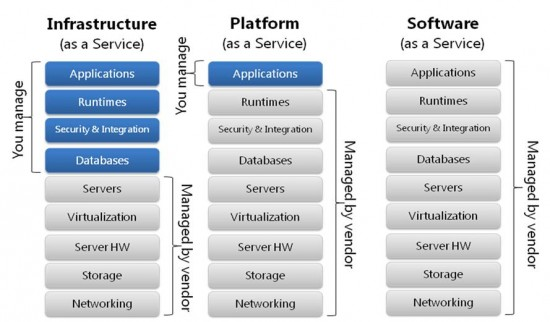
\includegraphics[width=\columnwidth, keepaspectratio]{_imagenes/Modelo_servicios.jpg}
    \caption{Mar Atlántico.} \label{fig:Modelo_servicios}
\end{figure}

\begin{description}
    \item[Cloud Software as a Service (SaaS).] El servicio provisto al usuario consiste en consumir una aplicación que es ejecutada en la nube, a demanda, vía multitenencia. Las aplicaciones que suministran este modelo de servicios son accedidas mediante un navegador web o de cualquier aplicación diseñada para tal efecto.
        El usuario no tiene control sobre la infraestructura de la nube, siendo transparente para el y eliminando la necesidad de instalar la aplicación en sus propias computadoras evitando costes de hardware y mantenimiento.

    \item[Cloud Platform as a Service (PaaS).] El servicio provisto al usuario consiste en utilizar la infraestructura de la nube para ejecutar aplicaciones desarrolladas por el usuario o adquiridas a terceros.
        Es el encapsulamiento de una abstracción del ambiente de desarrollo con sus modelos.
        El usuario no maneja ni controla la infraestructura de la nube, pero tiene control sobre la aplicación que es ejecutada y también sobre la configuración de entorno de ejecución de la aplicación.

    \item[Cloud Infraestructure as a Service (IaaS).] El servicio provisto al usuario consiste en la infraestructura de ejecución. El usuario es capaz de ejecutar código arbitrario, controla el sistema operativo y todas las aplicaciones de la nube.
        El hardware está virtualizado en la nube y se provee al usuario recursos como servidores, almacenamiento, redes, etc. Cada vez es mas adoptado este modelo, sobre todo por una gran cantidad de startups que lo utilizan por no poder permitirse tener datacenters propios. Provee mecanismos fáciles para que los desarrolladores interactúen con el IaaS generalmente creando máquinas virtuales. La interacción de las aplicaciones con IaaS suele ser a través de SOA con contratos de servicios, mediante WSDL o REST.
        Está dirigido a empresas que desean delegar la implantación de sus sistemas  en la infraestructura hardware de un proveedor externo, o servicios de almacenamiento externo, copias de seguridad de sus datos, cálculos complejos que requieran software de elevadas prestaciones, entre otros. El proveedor les permitirá gestionar dichos sistemas en un entorno virtualizado.

\end{description}

\section{Modelos despliegue}

Existen tren modelos de despliegue o tipos de cloud, el tipo de cloud a adoptar se debe definir en base a quien va a poder acceder a los servicios y a quien va a gestionar la infraestructura. Los tipos son privadas, públicas e híbridas y a continuación se explican cada una de ellas.

\begin{description}
    \item[Cloud privado] Una nube privada es aquella en la que solamente una organización, utilizando tecnologías como virtualización, tiene acceso a los recursos que se utilizan para implementar en la nube. Podría compararse con los datacenter que disponen algunas empresas, con infraestructura y máquinas propias dimensionadas en base a la demanda esperada. Mediante la virtualización se puede añadir a las características de los datacenters los beneficios del cloud como la agilidad de provisión o cierto nivel de elasticidad.
        La principal ventaja es que generan seguridad para los clientes, ya que no comparten recursos con otros usuarios. La capacidad de elegir el proveedor permite a los clientes seleccionar los recursos tecnológicos que mejor se adapten a sus necesidades técnicas y económicas.
        La desventaja que presenta este modelo es que al ser infraestructuras dedicadas al autoconsumo, el "pago por uso" no es un beneficio directo, ya que los recursos no utilizados no se revenden a otras organizaciones.
        Así, las nubes privadas están especialmente orientadas a organizaciones con alta concentración de recursos y sistemas tecnológicos, tales como entidades bancarias, Administración Pública, entornos de investigación y desarrollo, consultorías y asesorías legales, tecnológicas o de negocio, etc.

    \item[Cloud público]
        Una nube pública (o Cloud multi-tenant) se caracteriza por ofrecer recursos  sobre infraestructuras compartidas entre múltiples clientes. A estos recursos el cliente accede a través de internet o mediante conexiones VPN. La infraestructura es proporcionada con todas las ventajas del modelo de consumo de Cloud (pago por uso, aprovisionamiento ágil, elasticidad, etc.) beneficiándose además de las economías que se aplican al amortizar la infraestructura global con múltiples clientes.
        La ventaja más clara es que se adquiere poder de procesamiento y almacenamiento sin requerir inversión inicial, ya que se paga por lo que se usa. La desventaja se encuentra por el acceso al servicio a través de terceras empresas. También puede ser difícil integrar estos servicios con otros sistemas propietarios.

    \item[Cloud híbrido]
        Es un despliegue que combina recursos de cloud públicos y privados. Surge de la necesidad de los clientes de a pesar de tener su propia infraestructura buscar aprovechar las ventajas de los servicios de proveedores externos.
        Esto permite a una empresa mantener el control sobre las aplicaciones críticas para su negocio y aprovechar al mismo tiempo las posibilidades ofrecidas por los servicios ofertados por la nube en aquellas áreas donde resulte más adecuado. Aportan agilidad y reducción de costes sacrificando algo de control pero son una solución compleja, ya que requiere coordinación entre una infraestructura propia con otra gestionada por otro entorno.

\end{description}

\section{Ventajas y desventajas del cloud}
\subsection {Ventajas del uso de cloud}
Las ventajas que presenta el uso de la nube son varias y están asociadas a las necesidades y capacidades del cliente. Una de las ventajas más notables es como se mencionó es el modelo "paga por lo que uses", mediante la utilización de este modelo se presenta una ventaja al cliente, ya que paga solamente los recursos que utiliza y el proveedor tiene la ventaja que puede brindar los recursos que no son utilizados a otros clientes. A esto también le podemos sumar el ahorro por los gastos de infraestructura y mantenimiento. \\
El uso del cloud permite a Empresas no tan desarrolladas poder competir en cuanto a uso de tecnologías con otras más desarrolladas, teniendo acceso a últimas tecnologías y equipos costosos que sin el uso de la nube no podrían tenerlos.

Los datos pueden ser accedidos desde cualquier parte del mundo y con un acceso tolerante a fallos, lo que es beneficioso para los clientes que desean poder acceder a sus datos en todo momento.
Otra ventaja importante es la escalabilidad, en el uso de cloud la escalabilidad es transparente al cliente y en caso de necesitar más recurso de procesamiento o almacenamiento el proveedor se lo dará casi en tiempo real.
Se adecua al tiempo de mercado, por eso es utilizado por una gran cantidad de pequeñas empresas que recién comienzan, ya que sin la necesidad de una gran inversión pueden comenzar a trabajar tempranamente.

\subsection {Desventajas del uso de cloud}
Si bien como mencionamos anteriormente son muchas las ventajas que presenta el uso del cloud, también existen posibles desventajas.
La más clara tal vez es la privacidad, para muchos clientes es difícil confiar su información sensible a terceros dejando de tener control sobre ellos.
Otra desventaja es la disponibilidad, si bien se encuentra en la sección ventajas, también es una desventaja, ya que la disponibilidad tiene una fuerte dependencia con internet, sin internet no hay nube. También porque es el proveedor el encargado de proveer disponibilidad, pero si su tolerancia a fallos falla el cliente no puede hacer nada hasta que el proveedor lo solucione, existe una dependencia entre la disponibilidad y el proveedor.
Otra desventaja es que si un cliente desea cambiar de proveedor por cualquier motivo, no se puede garantizar el perfecto funcionamiento de su sistema. Esto se da porque no existe un estándar entre implementaciones de la nube por lo que la compatibilidad no está garantizada.

\section{Arquitecturas en la nube}
Para poder sacar provecho a una infraestructura escalable es de vital importancia que la arquitectura sea escalable. La nube está diseñada para proporcionar escalabilidad desde un punto de vista conceptual, sin embargo no se podrá aprovechar toda la escalabilidad de la infraestructura si la arquitectura del sistema no es escalable. Ambas deben trabajar mano a mano, debiendo identificarse los cuellos de botella y adecuando la misma con el objetivo de aprovechar la infraestructura escalable. A continuación se listan algunas de las características que se deben tener en cuenta a la hora de diseñar una arquitectura escalable:

\begin{itemize}
\item El aumento de recursos deriva en un aumento proporcional del rendimiento.
\item Un servicio escalable es capaz de gestionar la heterogeneidad.
\item Un servicio escalable es eficiente desde un punto de vista operativo.
\item Un servicio escalable es sólido.
\item Un servicio escalable debe ser más rentable cuando crece
\end {itemize}

La elasticidad dentro de una arquitectura es una noción pura del paradigma cloud, ya que la idea de poder contar con nuevos recursos en cuestión de minutos era imposible. La informática de nube optimiza el proceso de adquisición de los recursos necesarios. Ya no hay que realizar pedidos con antelación ni conservar hardware no utilizado. Ahora, los arquitectos de
la nube pueden solicitar los recursos que necesitan minutos antes de necesitarlos o automatizar el proceso de obtención, aprovechando la enorme escalabilidad y el rápido tiempo de respuesta.
La tolerancia a fallos y confiabilidad también son características deseables en arquitecturas cloud. La tolerancia a fallos es la capacidad del sistema de recuperarse y volver a un estado estable ante eventuales errores. La confiabilidad es disponer del correcto funcionamiento de todos los componentes al trabajar en conjunto.



\section{Ejemplo Cloud - Microsoft Azure}

Azure es la plataforma en la nube de Microsoft. Es una colección creciente de servicios integrados (proceso, almacenamiento, datos, red y aplicaciones).
Provee servicios siguiendo los modelos SaaS, PaaS e IaaS y la eficaz combinación de los servicios administrados y sin administrar permiten crear, implementar y administrar aplicaciones para obtener una buena productividad. Permite la posibilidad de tener un despliegue híbrido. Es abierto y flexible admitiendo cualquier sistema operativo, lenguaje, herramienta y marco, ya sea Windows, Linux, SQL Server, Oracle, C sharp o Java. Además, pone a su alcance lo mejor de los ecosistemas de Windows y Linux, por lo que puede se pueden crear excelentes aplicaciones y servicios que funcionan con cualquier dispositivo.
La plataforma Azure es más que servidores virtuales en varios centros de datos distribuidos estratégicamente. En la figura (\ref{fig:architectureazure}), se expone la arquitectura de la plataforma Azure y a continuación se detallan en cada uno de los mismos.

\begin{figure}[h!]
    \centering
    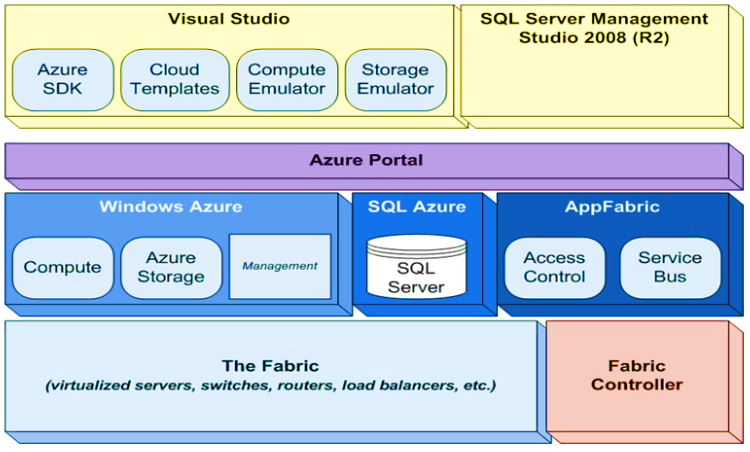
\includegraphics[width=\columnwidth, keepaspectratio]{architectureazure}
    \caption{Arquitectura de la plataforma Azure}   \label{fig:architectureazure}
\end{figure}



\begin{description}
    \item [The Fabric.] Se refiere principalmente a los componentes físicos que hacen posible la interoperabilidad entre sistemas, algunos de ellos como: servidores, switches, routers, etc. Fabric puede ser un sinónimo de centro de datos Microsoft.

    \item [Fabric Controller.] Esencialmente es software que opera bajo el modelo de controladores, utiliza drivers para cada componente de la fábrica además de administrar la implementación de servicios y almacenamiento de datos.

    \item [Windows Azure.] Se puede ver como el sistema operativo de la nube y se divide en tres servicios:
          \begin{itemize}
              \item Compute : Es el ambiente de ejecución donde aplicaciones y servicios ejecutan procesos computacionales, cualquier cloud service que se publique en Azure, se ejecutará aquí.
              \item  Storage : Es el ambiente para almacenar datos, se refiere a los tipos de almacenamientos en la nube (tablas, colas y blobs).
              \item Management : Infraestructura automatizada y administrada de los servicios en la nube.  El servicio de management es el fabric controller más otras funcionalidades.
          \end{itemize}

    \item [SQL Azure.] Es el sistema de gestión de base de datos relacional en la nube, es una versión modificada de SQL Server 2008.

    \item [AppFabric.] Es un componente clave que ofrece tres servicios:

          \begin{itemize}
              \item Access Control: Autenticación y permisos hacia las aplicaciones.
              \item  Service Bus: Mensajería segura y conectividad dentro y fuera de la nube.
              \item Caching Service: Cache para aplicaciones Azure.
          \end{itemize}

    \item [Portal Azure.] Portal web que permite la administración de todos los recursos que ofrece la plataforma Azure.

    \item [Herramientas.] Ambientes de desarrollo para la implementación de soluciones en la nube como Visual Studio o SQL Server Management Studio.

\end{description}

Los servicios son provistos mediante servicios REST mediante una REST API permitiendo acceder a los servicios a través de una plataforma web o consola. La configuración y control de los servicios se puede realizar a través del portal web Microsoft Azure Portal, con una interfaz sencilla y amigable, facilitando el uso a los usuarios y pudiendo accederla desde cualquier browser. De este modo el usuario no necesita instalar ningún componente para poder configurar y controlar los servicios. En cambio si se desea desarrollar aplicaciones para Azure si es necesario instalar ciertos componentes para la correcta depuración de la aplicación.


\subsection {Modelos de ejecución}
En Azure existen tres modelos de ejecución para proveer servicios al cliente. Ellos son Web Sites, Cloud Services y Virtual Machines. Cada modelo provee a su vez un conjunto de servicios y la elección de cual usar  por parte del cliente depende de las necesidades del mismo. A continuación detallamos cada uno de los mismos.

\begin{description}
\item [Virtual Machines.] Permite crear y usar máquinas virtuales en la nube y así provee IaaS.

\begin{figure}[h!]
    \centering
    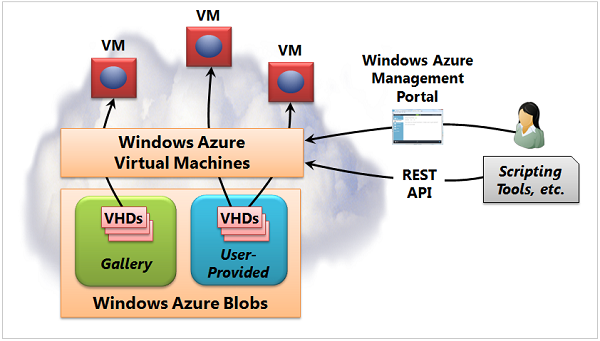
\includegraphics[width=\columnwidth, keepaspectratio]{_imagenes/azure_virtualmachines}
    \caption{Máquinas virtuales en Azure para proveer IaaS} \label{fig:azure_virtualmachines}
\end{figure}

El usuario puede crear y controlar máquinas virtuales desde el portal web o utilizando la REST API que mencionamos anteriormente. Al crear  una máquina virtual se debe elegir un disco duro virtual (VHD). Para esto existen dos opciones, una es que el usuario suba su propio VHD y la otra es usar uno nuevo que provee Microsoft en la galería de máquinas virtuales. Estos discos se guardarán en  Azure Blobs, se presentarán estos componentes más adelante. Los VHDs en la galería cuentan con imágenes de sistemas operativos Windows y Linux con productos ya instalados. Entre las configuraciones posibles se encuentran Windows Server, Linux servers, SQL server, BizTalk Server, SharePoint Server. También se debe seleccionar el tamaño que tendrá la máquina virtual, para esto se brindan configuraciones de memoria y cores los cuales debe seleccionar el usuario. Las configuraciones posibles son:

\begin{itemize}
\item Extra Small, con core compartido y  768MB de memoria.
\item Small, con 1 core y 1.75GB de memoria.
\item Medium, con 2 cores y 3.5GB de memoria.
\item Large, con 4 cores y 7GB de memoria.
\item Extra Large, con 8 cores y 14GB de memoria.
\item A6, con 4 cores y 28GB de memoria.
\item A7, con 8 cores y 56GB de memoria.

\end {itemize}
Por último se debe configurar sobre que datacenter correrá la máquina virtual creada siendo Estados Unidos, Asia o Europa las opciones.\\
Luego de creada la máquina virtual el pago se realiza por hora de trabajo.

\item [Web Sites.] Utiliza el modelo PaaS y permite desarrollar, deployar y escalar aplicaciones web. Se utiliza cuando el usuario no necesita tener control sobre la máquina virtual donde corre su aplicación, delegando dicho control a Azure.

\begin{figure}[h!]
    \centering
    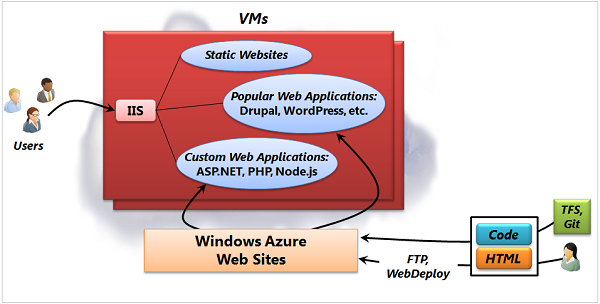
\includegraphics[width=\columnwidth, keepaspectratio]{_imagenes/azure_websites}
    \caption{WebSites en Azure para proveer PaaS} \label{fig:azure_websites}
\end{figure}

Web Sites de Azure permite tanto la creación de nuevos sitios, como la migración de sitios ya existentes. En ambos casos es posible configurar el escalado del sitio según los criterios definidos.
El usuario tiene la posibilidad de optar si desea utilizar una máquina virtual para el solo o una compartida y provee templates, frameworks y herramientas para el fácil y rápido desarrollo de aplicaciones web. La tecnología da soporte para la creación de aplicaciones usando ASP.NET, PHP, Node.js y Python.
Aplicaciones creadas en WebSites también pueden usar otras funcionalidades de Azure como Service Bus, SQL Database, y Blob Storage.\\
Para la publicación del sitio se puede realizar mediante FTP, FTPS o tecnología de Microsoft para deploy. También desde sistemas de source control como Git, GitHub, Bitbucket, Dropbox, Team Fundation Server.

Azure Websites no solo funciona con aplicaciones web, también se pueden realizar tareas de cómputos utilizando WebJobs.


\item [Cloud Services.] Cloud Services es otro ejemplo de PaaS. Al igual que WebSites está desarrollado para soportar aplicaciones escalables. Si bien los clientes no tienen control absoluto sobre las máquinas virtuales, tienen mas control que usando WebSites.



La tecnología provee dos opciones de virtualización, una basada en web roles que ejecutan un similar a Windows Server con IIS mientras que la otra opción es ejecutar web roles, también similar a Windows Server pero sin IIS. Por ejemplo una aplicación simple puede ejecutar solo en un web role pero si la aplicación es compleja además de ejecutar en web role se puede pasar trabajo a worker roles.

\begin{figure}[h!]
    \centering
    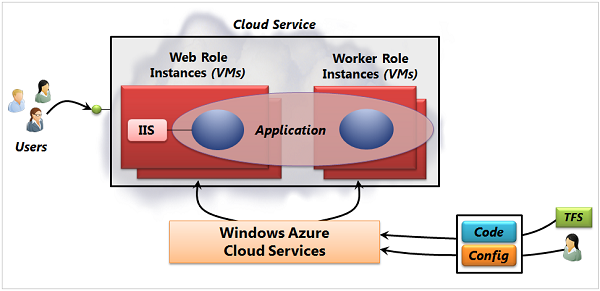
\includegraphics[width=\columnwidth, keepaspectratio]{_imagenes/azure_cloudservices}
    \caption{Cloud Services en Azure} \label{fig:azure_cloudservices}
\end{figure}

\end{description}


\red{faltan referencias}
La elección del modelo a utilizar es fuertemente dependiente de las características del problema a resolver. Si se desea por ejemplo una aplicación con poca configuración y acceso a base de datos, Web Sites es la opción que mejor se adapta a estas necesidades. Por otro lado, si se desea crear una arquitectura con mas de una capa que ejecute aplicaciones con gran nivel de computo y específicas condiciones de escalado, Cloud Services es la opción correcta. En cambio, si se desea instalar en el cloud una aplicación que requiere gran configuración del sistema operativo subyacente, la mejor opción en este caso sera utilizar Virtual Machines.

\subsection {Modelos de almacenamiento}
\red{faltan referencias}
El acceso a datos en Azure se realiza mediante servicios RESTful pudiendo realizar llamados desde consola o aplicación web. Desde el portal también se pueden crear las cuentas de almacenamiento de forma rápida y sencilla. La cantidad de cuentas de almacenamiento que puede crear el usuario está limitado por el tipo de cuenta de Azure que el usuario posee. Azure provee cuatro opciones para el manejo de almacenamiento, blobs, tables, queues y drives o unidades.

\begin{description}

    \item [Blobs.] Un Blob es un archivo de cualquier tipo. Existen dos tipos, Block y Page Blob. Block Blob es optimizado para el uso de streaming de datos mientras que Page Blob es optimizado para la realización de operaciones de lectura / escritura.Los blobs se alojan en Containers, pudiendo tener una cantidad ilimitada de Blobs respetando los tamaños máximos de almacenamiento permitido. El acceso a un Blob se realiza utilizando la URL con el formato
          http://[storageAccount].blob.core.windows.net/[container]/[blob]

          \red{faltan referencias}
    \item [Tables.] Permite almacenar gran cantidad de datos estructurados. Una tabla es definida dentro de una cuenta de almacenamiento pero no dentro de un Container y esta conformada por un conjunto de entidades. La diferencia entre las tablas de Azure y las de base de datos relacionales es que las tablas de Azure no posee esquema de entidades, por lo que entidades de una misma tabla pueden poseer distintas propiedades.

          \red{faltan referencias}
    \item [Queues.] Permite almacenar una gran cantidad de mensajes que pueden ser accedidos utilizando llamados HTTP o HTTPS autenticados. Pueden actuar como una forma de enrutar trabajo entre los diferentes roles dentro de una aplicación de una forma durable y escalable.

          \red{faltan referencias}
    \item [Drives.] Son espacios NTFS donde podemos utilizar las APIs tradicionales de lectura y escritura. La diferencia de utilizar un servicio de drive o utilizar el drive de la máquina virtual es que el servicio de drive está disponible para todos los roles y preparado para escalar.


\end{description}

\subsection {HDInsight}
\red{faltan referencias}
HDInsight es un servicio de Azure que provee y despliega clústers de Apache Hadoop \cite{hadoop} en el cloud, brindando un framework para analizar, manejar y reportar grandes volúmenes de datos, ofreciendo así una implementación del model MapReduce de Apache Hadoop para el análisis de big data. Los clusters Hadoop en HDInsight utilizan una versión de Hortonworks Data Platform(HDP) y un conjunto de componentes de Hadoop de dicha distribución. En la versión actual de HDInsight, la 3.1,   la versión 2.1.7 de HDP y 2.4.0 de Apache Hadoop. En HDInsight el sistema de archivos de Hadoop (HDSF) se almacena como Blobs en un Container asociado al cluster en la cuenta de almacenamiento.\\

\begin{figure}[h!]
    \centering
    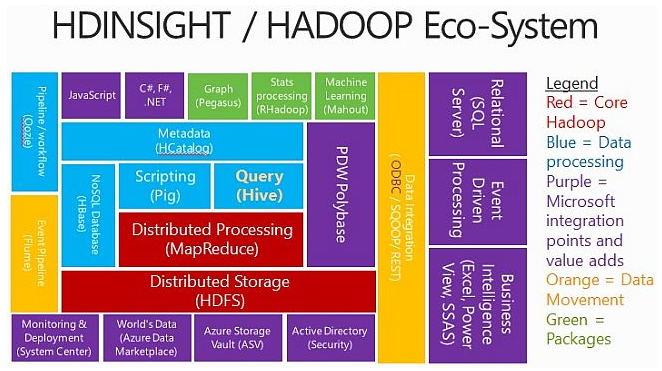
\includegraphics[width=\columnwidth, keepaspectratio]{HDInsight}
    \caption{Ecosistema HDInsight / Hadoop}
    \label{fig:HDInsight}
\end{figure}


\chapter{Descripción de la investigación}

En este capítulo\dots

\section{Frameworks}



\subsection{Spring}

Spring\dots

\subsection{Quarkus}

Quarkus is a full-stack, Kubernetes-native Java framework made for Java virtual machines (JVMs) and native compilation, optimizing Java specifically for containers and enabling it to become an effective platform for serverless, cloud, and Kubernetes environments.
\cite{WhatisQu51:online}\\

\subsection{Micronaut}



\subsection{helidon.io}


\chapter{Trabajos relacionados}

En este capítulo son incluidos  los trabajos de investigación relacionados, publicaciones, productos y libros al respecto de la utilización de Microservicios en arquitecturas distribuidas para el procesamiento de grandes volúmenes de datos.

\section{Artículos}

\paragraph{
\textbf{\emph{An Experimental Study on Microservices based Edge Computing Platforms}}
\cite{qu_experimental_2020}.
}

\paragraph{
Motivado por la arquitectura de microservicios y su aplicación en ciudades inteligentes,
múltiples políticas de despliegue en plataformas de computación de borde (EDGE) fueron investigadas en este artículo. Se argumentó contra las máquinas virtuales, haciendo referencia a estudios de IBM en cuanto al consumo de recursos, comparando ejecuciones con Spark \cite{ApacheSpark} utilizando grandes volúmenes de datos. En cuanto al uso de contenedores se tomó en cuenta un estudio en el área big data sobre la interferencia causada entre contenedores vecinos ejecutando microservicios sobre big data \cite{BigDataWikipedia}.  
}

\paragraph{
Si bien no es mencionado explícitamente, la aplicación a big data depende del escalado de los datos de entrada. La arquitectura planteada se define en contraposición a una arquitectura típica de big data. Por ese motivo fue uno de los artículos seleccionados como trabajo relacionado.
}

\paragraph{
Para la investigación fueron utilizados contenedores docker. A través de pruebas experimentales en distintos escenarios se comparó el desempeño, considerando que la capacidad de recolectar y procesar los datos de borde es la clave.
Se evaluó por parte de los investigadores si es apropiado ejecutar múltiples microservicios dentro de un contenedor considerando la performance del dispositivo.
En caso de que fuese viable, se identificaron que tipos de microservicios eran agrupables en cuanto al perfil de consumo de recursos.
Fue verificado si el efecto de interferencia al ejecutar múltiples microservicios en una infraestructura de computación de la niebla (FOG), es el mismo que en EDGE. Cabe mencionar que la computación de niebla (también conocida como redes en la niebla o niebla)
es una infraestructura de computación descentralizad donde las aplicaciones están distribuidas en el lugar más eficiente entre la fuente de datos y la nube.
La distribución de microservicios fue comparada tomando en cuenta la regla de un proceso por contenedor (o un contenedor por servicio) 
\cite{cont_por_serv} 
contra las limitaciones de recursos en EDGE en términos de computación y memoria.
\cite{webfog}.
}

\paragraph{
Como ambiente fue utilizado para FOG una máquina de escritorio 4,5 GHz Intel Core TM (4 núcleos),
4 GB DDR3 RAM y 50G HHD, sobre Ubuntu 16.04. Y para EDGE Raspberry Pi 4, Quad Core Cortex-A72 (ARM v8) 1,5 Ghz,
4 GB LPDDR4 RAM y 32 GB microSD card, sobre Raspbian GNU/Linux.
 Se plantearon cuatro casos a evaluar.El primero, una única instancia de microservicio por contenedor y solo un contenedor ejecutándose en el host. 
 El segundo, múltiples instancias de microservicios en un contenedor y solo contenedor ejecutándose en el host. El tercero cada contenedor albergó una única instancia de microservicio y múltiples contenedores ejecutándose en el host. El cuarto cada contenedor albergó una única instancia de microservicio y múltiples contenedores ejecutaron en el host, con la limitante de la utilización de cgroups para limitar el acceso al sistema durante el test.
}

\paragraph{
 La performance de la CPU se evaluó con Linpack benchmarks 
\cite{LINPACKBenchmarksWikipedia}, la performance de la memoria con STREAM benchmarks 
\cite{STREAMBenchmarkAMD} 
y la del disco con Bonnie++ benchmark \cite{BonnieWikipedia}.
 Con las mencionadas herramientas de benchmarks y posibles configuraciones en los casos mencionados,
 se realizaron los test decidiendo según el resultado que flujo de test seguir.
 De esa manera se realizó la evaluación de las diferentes distribuciones en FOG y en EDGE, llegando a concluir, que en un ambiente de computación de borde el ejecutar múltiples instancias de microservicios en un contenedor,
 tiene como ventaja una mejora en la performance en la mayoría de los casos.
 En contra partida, tiene como gran desventaja que al momento de escalar en contenedores se replican todos los microservicios desplegados en el contenedor
 y no solo los necesarios, por lo que resulta contraproducente en recursos. 
 En cuanto al uso de la memoria no se verificaron diferencias significativas, 
 salvo cuando microservicios similares dentro de un contenedor competían por el mismo recurso como la entrada salida del disco.
}

\paragraph{
  Al final del articulo los autores plantearon realizar un prototipo a mayor escala con los datos relevados.
 }
\subsection{\textbf{
        \emph{Microservice-Oriented Platform for Internet of Big Data Analytics: A Proof of Concept}
    }
}

El artículo "Microservice-Oriented Platform for Internet of Big Data Analytics: A Proof of Concept"\cite{li_microservice-oriented_2019}, se basó en que los dispositivos de internet de las cosas (su sigla en inglés IoT) generan numerosos datos desde cualquier lugar y en cualquier momento. Se planteó demostrar que no siempre es necesario centralizar y analizar los datos acumulados como plantean las implementaciones tradicionales de análisis de grandes volúmenes de datos (su sigla en inglés BDA), en donde son trasmitidos grandes volúmenes de datos hacia el sistema centralizado, pudiendo reducir el costo de la transmisión preprocesandolos de manera anticipada. Se definió en el artículo la sigla IoTBDA para identificar el concepto planteado de BDA implementado sobre IoT.\par

Los autores plantearon una plataforma orientada a microservicios inspirados en la infraestructura definida por el software (su sigla en inglés SDI).
Se indicó que de acuerdo a las especificaciones funcionales de las plataformas BDA, generalmente se combina el procesamiento de datos en conjunto con la gestión de los recursos informáticos. Incluso el almacenamiento de los datos en ocasiones es parte de la plataforma, dando lugar a un sistema que requiere un esfuerzo significante en cuanto a configuración y manipulación.
En cuanto a la arquitectura basada en microservicios (su sigla en inglés MSA) fueron destacadas varias cualidades aplicadas a IoTBDA. Entre las cualidades se encuentra la posibilidad de descomponer sistemas monolíticos en múltiples sistemas de menor escala, perdiendo acoplamiento y brindado la posibilidad de escalar solo los servicios necesarios. Además la MSA brinda la posibilidad de dado problemas particulares no solo desarrollar microservicios para ese problema, sino que realizar microservicios reutilizables creándolos funcionalmente genéricos, o como plantillas de microservicios.\par

Las plataformas orientadas a MSA pueden ser orquestadas por microservicios, un conjunto de microservicios estándar o plantillas de estos. Esto último en particular es de interés para la realización del proyecto, puesto que es considerada la orquestación como uno de los temas esenciales a la hora de diseñar una MSA. Mediante diseños de MSA fue implantado IoTBDA. En un primer caso se planteó como arquitectura un conjunto de sensores a través de una instancia de observador, contra un único procesador central.\par

Los autores consideraron que la tecnología de contenedores que además de estar en una etapa creciente, permite el soporte para múltiples dispositivos de borde.
Los sensores que se mencionaron como componentes de borde de la IoTBDA no poseen una forma estándar de comunicación con otros sensores ni con los servidores, existiendo incompatibilidades y protocolos propietarios para asegurarse un mercado en contra de sus competidores. Exponiendo las diferentes tareas de procesamiento por microservicios a través de  interfaces en una API con un lenguaje unificado, que evitaría esos inconvenientes permitiendo que no se vea comprometida la heterogeneidad de los sensores de borde.\par

El caso de prueba incluyó la implementación del método de Montecarlo utilizando lógica orientada a microservicios.
En la  MSA se definieron tres elementos principales observadores, un procesador central y un aggregator.
Los observadores también llamados templates de microservicios son instanciados para una tarea específica.
Un procesador central que en principio funciona como splitter o sea divide todo el trabajo en piezas independientes y se lo asigna a cada observador.
Luego tomando los resultados este y los carga en el aggregator, el cual se recolecta los resultados globales para poder ser consultados de forma inmediata.
Como análisis conceptual, se estimó el valor de una integral doble mediante la aproximación utilizado el método de Montecarlo. Esto fue realizado para validar la solución de la arquitectura presentada y evaluar el funcionamiento de la misma como así su eficiencia. Se realizó el cálculo de aproximación a una integral por 10 millones de puntos aleatorios en un entorno distribuido y se comparó con una ejecución local sobre el mismo problema.
El procesador central efectuó la reducción de los datos o sea que existe cierta similitud con lo que sería un map reduce, donde el mapa de los observadores y reduciendo el procesador central dejando los resultados en el observation aggregator donde puede ser consultados a este de forma inmediata.\par

La conclusión fue que la lógica orientada a microservicios para el análisis convergente se ajusta más a las características de IoTBDA. Al ser considerada una topología de árbol para el análisis convergente (como un map reduce en cascada) se reduce el tamaño de la transmisión de datos.
Existe un paralelismo entre microservicios para el análisis convergente y la lógica de map reduce. Es posible descomponer en partes de problemas específicos como los mapas y los reduce para ser implementado por microservicios.
De esta manera se validan los modelos de arquitectura para IoTBDA identificando los sensores (como ser dispositivos móviles) como observers, optimizando el tráfico y recolección de datos a través de la arquitectura presentada como análisis convergente.
Mediante la prueba conceptual se determinó que mediante la convergencia intermedia (como plantea el análisis convergente)  disminuye en un 97\% la transmisión de datos y en la convergencia final y salva un 61\% de transmisión de datos. Lo cual hace muy atractivo este enfoque.\par











\paragraph{
    \textbf{\emph{Orquestación de servicios para el desarrollo de aplicaciones para big data}}
    \cite{orquestacion}.
 }

Uno de los temas importantes cuando se habla de micro servicios es la orquestación de los mismos. Y para ello se seleccionó este paper. 

Fueron introducidos los conceptos de microservicios aclarando que los mismos permiten replicar y distribuir logrando así altos niveles de escalabilidad se planteó la orquestación de contenedores sobre una arquitectura distribuida virtualizada. 

Llama la atención que al igual que otros papers fueron mencionados los conceptos de cloud computing en Internet de las cosas apuntando a smart cities, concepto que se desarrolló y se valoró. Concepto que puso desafíos como el de la heterogeneidad los dispositivos y las tecnologías involucradas, para lo cual hay que tener en cuenta la ubicuidad y la omnipresencia de los dispositivos. 
Para ello se planteó una plataforma de computación escalable, puesto que la convergencia de todos ellos requieren de que sea centralizados sus grandes  volúmenes de datos. 

Se mencionó que las características que hacen que los sistemas de cómputo convencionales no son los adecuados para big data por los tiempos de captura procesamiento y persistencia de los datos. Se hizo referencia que no se trata de recopilar datos y hacer análisis detallado, sino de hacer interpretaciones rápidas que orienten en la toma de decisiones a partir de datos de cualquier fuente, de cara a la implementación de un sistema big data como ser el de smart cities.


El paper trató un punto base de las arquitecturas de microservicios, que es la orquestación y por lo cual este paper fue seleccionado. Se indicó que construir aplicaciones de big data tiene como principal reto la necesidad de administrar esos recursos, conocer y planificar de qué forma van a escalar. 

Tradicionalmente las aplicaciones escalan verticalmente, donde frente a tener que resolver algún cuello de botella se dedica una mayor cantidad de recursos. 

Pero en el caso de arquitectura distribuidas basadas en big data se determinó que la escalabilidad debe ser horizontal, de modo que permita distribuir la carga de trabajo dinámicamente, tanto así como paralelizar las tareas. 
Se definió como escalabilidad horizontal la implicancia del balanceo de carga, aplicación de recursos, reinstalación sesión de recursos en tiempo real y optimización de su uso de forma que el usuario no perciba degradación de performance. 


Algo que fue aclarado y que deja de evidencia la necesidad de orquestación en este tipo arquitecturas, es enfáticamente el concepto de que los microservicios son independientes. 
Cada micro servicio no conoce lo que está ejecutando el otro microservicio por lo cual al tener una serie entidades independientes y al existir transacciones que dependan de todas ellas, es necesario contar con un módulo de orquestación. 
Es decir una entidad o un conjunto de entidades que pueda manejar la lógica que atraviesa todos los microservicios para identificar que se está ejecutando, en qué momento y que se debe ejecutar a continuación.
Que permita conocer el estado del sistema, poder consultar el mismo, acceder a estadísticas entre otros. 


Para desarrollar esta arquitectura de microservicios se utilizaron contenedores, de tal manera que cada microservicio se ejecuta en un contenedor el cual contiene todas sus dependencias.

A través de estos contenedores dado que los mismos son livianos y portables, además de que son independientes al hardware y al software en donde se crearon, es que se puede armar una arquitectura distribuida con ellos. 

Los contenedores generan una baja sobrecarga e introducen menos overhead que las máquinas virtuales convencionales. 


Se aclaró la diferencia entre la máquina virtual y el contenedor explicitando que ambos son sistemas autocontenidos que tienen como principal diferencia que una máquina virtual necesita contener todo el sistema operativo mientras que un contenedor aprovecha el sistema operativo en el cual se ejecuta. 


Fue indicado que una de las formas de escalar horizontalmente es mediante el uso de múltiples nodos y que para lograrlo es necesario abstraerse de la complejidad de la plataforma, y esto es posible mediante el uso de clusters de contenedores.


Donde cada nodo en el cluster es un servidor virtual y puede tener múltiples contenedores con una semántica común,
por lo que una aplicación puede estar formada por un grupo de estos contenedores, lo cual le permite escalar a través de múltiples nodos. 
 

Para trabajar de esta manera se necesita administrar y coordinar esos contenedores. 
Y para ello es posible realizar dos tipos administración u organización, en donde se señalaron como opciones, la orquestación y la coreografía. 

Fueron comparados los conceptos de orquestación y coreografía de servicios. Se indicó que orquestación (como ya se mencionó) implica que hay una entidad central que conoce todo el funcionamiento del sistema, y conoce todas las ejecuciones que están realizando todos los servicios. Mientras que los servicios coreografiados conocen exactamente cuando ejecutar sus operaciones y con quien debe interactuar, lo cual les quita independencia y es va en contra del paradigma de microservicios.


Solamente la entidad central es la encargada de la orquestación y conoce cuál es la meta a conseguir por lo cual la orquestación se realiza mediante definiciones explícitas de las operaciones y el orden de invocación.


Se resumió el concepto de orquestador de contenedores, como una herramienta que permite crear un cluster de alta
disponibilidad de virtualización de contenedores, dotándolo de un sistema orquestación dinámica de servicios en el ámbito de múltiples servidores.

Se mencionaron una serie de productos los cuales permiten realizar la orquestación de contenedores.
Cómo ser Kubernetes, Marathon Mesos \cite{matathonMesos}, Conductor\cite{conductor}y Docker Swarm\cite{dockerSwarm}. 
Como tecnología de contenerización se decidió trabajar con Docker para implementar la orquestación se eligió  Docker Swarm. 
 
 
El orquestador posee una arquitectura maestro esclavo. Cabe destacar que no es una típica arquitectura maestro esclavo. En este caso las entidades no son únicas, sino que el maestro es un nodo con un conjunto de contenedores, por lo cual frente a la caída de un contenedor se levanta otro y se sigue ejecutando obteniendo así alta disponibilidad de maestros.
En cada esclavo funciona un agente que recibe las tareas y entrega al nodo maestro los informes con el avance. 
Para el caso estudio se optó como forma de acceder rápidamente a los datos, replicar los mismos. 
Esto es según síndico una solución en la cual se puede lograr balanceo de carga, procesamiento concurrente y paralelización. 


Para el caso de estudio, se creó mediante la configuración del cluster Swarm, una estructura formada por un maestro (manager) y cuatro esclavos (workers). 
Con dicha configuración se acceden a las réplicas a través de un frontend web.

Se mencionó Docker Compose\cite{dockerCompose} como una herramienta que permite armar una aplicación con tantos componentes como sean necesarios, para posteriormente orquestar la misma en el cluster. 


Como conclusión se planteó que trabajar en el desarrollo de aplicaciones de big data permite lograr escalabilidad mediante réplicas de la aplicación, lo cual es fundamental cuando se trabaja con sistemas que demandan restricciones de tiempo. 
Ese escalamiento puede aumentar o disminuir de forma elástica como consecuencia de la orquestación de sistema. 


Se mencionó que el uso de contenedores permite la interoperabilidad entre todos los microservicios así como la independencia de las tecnologías internas de cada microservicio, 

No se está de acuerdo con ese concepto, porque se puede tener interoperabilidad entre los microservicios sin estar dentro de contenedores, y la independencia de tecnologías internas de cada micro servicio la determina la arquitectura de microservicios de por sí. Y como son aplicaciones que solamente deben exponer servicios a través de HTTP, los mismos pueden ser implementados en diferentes lenguajes, sobre diferentes plataformas y sobre diferentes sistemas operativos.

\subsection{
    \textbf{\emph{Automation of distributed data management in applied
            microservices package for scientific computations
        }
    }
    \cite{oparin_automation_2020}.
}

En el marco de la conferencia
\textbf{The International Workshop on Information, Computation, and Control Systems for Distributed Environments},
fue presentado el artículo en cuestión en el cual se ofrece conjunto de herramientas especializadas para automatizar la gestión del conocimiento en
la creación de microservicios y la acumulación de datos, aplicado a
cálculos científicos en un entorno informático híbrido.\par

Los autores se enfocaron en la utilización de microservicios para la automatización de la creación y adaptación de aplicaciones existentes para proveer la habilidad de resolver problemas complejos dentro de algún subject domain (SD).
Este artículo fue seleccionado porque utiliza una arquitectura de microservicios automatizada y como parte de una
lógica customizable.\par

El concepto arquitectónico base de microservicios que se utilizó es Applied Microservice Package (AMP),
el cual según se indicó provee de un camino efectivo para la computación científica distribuida.\par

El modelo computacional AMP se encuentra representado por un conjunto de pequeñas piezas con bajo acoplamiento,
implementado con microservicios.\par

La inteligencia de las AMP esta basada en el modelo de SD,
que se comprende como una colección de información sobre los objetos SD y las relaciones entre ellos.
De esta manera el conjunto de herramientas desarrolladas automatiza la creación y actualización
de las bases locales de conocimiento del los agentes distribuidos. Las bases locales de conocimiento
son creadas de mediante el uso de interfaces administradas por estos agentes.
El sistema utiliza dicho conocimiento para testear las actualizaciones de los microservicios,
además de proveer sincronización y persistencia de los datos calculados.\par

Se mencionó que el uso de arquitectura de agentes en conjunto con microservicios provee de una oportunidad práctica
para implementar mecanismos de interacción semántica de los agentes en una red P2P.
Las ventajas de las redes P2P mencionadas fueron escalabilidad, minimización de costos de comunicación,
autorganización adaptabilidad, tolerancia a fallos y autobalance de carga.
De esta manera fue evitada la centralización del acceso a los de servicios.\par

LA validación de la solución se realizó mediante el desarrollo de una solución que se basó en contratos Booleanos (BDS) para Sistemas Dinámicos,
se validó la solución propuesta.
BDS tiene aplicación en el campo de la bioinformatica.\par

Se diseñó un sistema que además de tener un administrador de autorización y manejo de archivos tiene
Administración de sincronización, Wizard de Creación, Wizard de Configuración, Wizard de Test, Wizard de Actualización. Donde la administración de sincronización, administra la sincronización de las bases de conocimientos locales. El Wizard de Creación, automatiza la creación de nuevos servicios basados e en plantillas estándar,
populando la base de conocimiento local. El Wizard de Configuración, automatiza el alta de parámetros de los agentes,
para definir la relación de los agentes con las funcionalidades de los microservicios. El Wizard de Test, automatiza el testeo de los paquetes desplegados, y la interacción de los agentes con los microservicios. El Wizard de Actualización, automatiza la actualización de agentes y microservicios desde repositorios externos y locales.
Se accede a todo el paquete administrativo a través de una interfaz web.\par

El artículo explicitó el funcionamiento de la actualización y testeo de microservicios,
en el que se aclaró que en caso de que el microservicio estuviera involucrado
en un proceso en ejecución queda bloqueada la actualización hasta que esté se complete.
De igual manera se bloquea el acceso a usuarios a procesos que involucren el microservicio a actualizar y testear.
En cuanto al ejemplo práctico de la plataforma fue desarrollado AMP para el estudio cualitativo de BDS,
el cual se dividió en los siguientes grupos de microservicios creación de modelos booleanos, validación de los contratos booleanos, pre y postprocesador del procesamiento.\par

La conclusión fué que el conjunto de herramientas provee varios modelos de datos,
sincronizando entre recursos locales y de la nube, microservicios actualizados y testeados.
Las pruebas realizadas confirmaron la efectividad de la solución para resolver
problemas prácticos significativos de carácter científico. Como también que la automatización y administración
mejora la productividad del desarrollador, creando y actualizando AMP, como también la del usuario final en la
solución de problemas de investigación de BDS.\par

\subsection{Emerging Technologies in Computer Engineering: Microservices in Big Data Analytics: Second International Conference, {ICETCE} 2019, Jaipur, India, February 1–2, 2019, Revised Selected Papers
}

El libro "Emerging Technologies in Computer Engineering: Microservices in Big Data Analytics: Second International Conference, {ICETCE} 2019, Jaipur, India, February 1–2, 2019, Revised Selected Papers"\cite{somaniEmerging2019} presentó un conjunto de veintinueve papers seleccionados y revisados relacionados con big data y microservicios,
donde se encuentran temas tan variados como ser detección de tumores o predicción de choques con icebergs, pasando por las redes sociales y los incendios forestales.
Dentro de los papers seleccionados además de big data y microservicios se encuentran tecnologías como IoT, Blockchain,
redes neurales, machine learning, detección de ciber ataques, smart dust,
Se incluyen algunos de dichos papers.\par

\paragraph{
    \textbf{\emph{An Efficient and Adaptive Method for Collision
    Probability of Ships, Icebergs Using CNN
    and DBSCAN Clustering Algorithm}
    }
    \cite[pág. 20]{somani_emerging_2019}.
}

Los autores crearon un modelo para predecir las colisiones entre barcos e icebergs, 
tomando en cuenta la ubicación y velocidad del barco, y la cantidad de icebergs en la zona.
Para calcular la probabilidad de que un barco colisione con un iceberg 
se utilizó el teorema de Bayes de probabilidad condicionada, analizando imágenes con la técnica CNN (Convolution neural network).
Se entrenó una inteligencia artificial (AI) utilizando CNN, mediante varios test de imágenes la AI fue aprendiendo 
y mejorado la precisión.

Utilizando agrupamiento DBSCAN se particionó las zonas a escanear y se ponderaron
las mismas mediante conteo y valores condicionales. Los atributos que se suministraron al teorema de Bayes fueron 
velocidad del Barco, ubicación, y precencia de icebergs (obtenida con CNN). 
 
Como conclusión se destacó que el trabajo aparentó ser eficiente en predecir
una medida precisa de  las probabilidades resultantes.
Debido a que la predicción de icebergs utilizando imágenes es ineficiente se agregó una capa de una interfaz Bayesiena
para definir la probabilidad de colisión. Después de la predicción se utilizó 
la técnica de agrupamiento para crear grupos que representan zonas seguras e inseguras para los barcos.


\subsection{Smart Judiciary System: A Smart Dust
            Based IoT Application
}

Este artículo "Smart Judiciary System: A Smart Dust
Based IoT Application"\cite[pág.128]{somaniEmerging2019}, fue elegido debido a que el concepto de tener sensores lo suficientemente pequeños como para llamarlos polvo, da para pensar en nuevas aplicaciones de tecnología IoT, y son una invitación a utilizar la imaginación.
El mismo plateó que la tecnología presentada mejoraría la precisión, transparencia e inteligencia de las posibles aplicaciones involucradas.
El artículo planteó como base la utilización de la tecnología de polvo inteligente para la detección de actividades criminales.
Buscando con su aplicación la reducción de crímenes. Lo que actualmente se puede apreciar en sistema de vigilancia mediante redes de cámaras dispuestas
para desalentar la actividad criminal, o sea con similares características pero utilizando estos sensores minúsculos.\par

Los autores mencionaron que los militares norteamericanos invierten en la investigación de tecnologías como las microelectromecanicas (MEMS) con aplicación en vigilancia. Plantean que en el futuro nubes de pequeños sensores podrán ser trasladadas en el aire y que otras aplicaciones de esta tecnología pueden ser la construcción de puentes, el seguimiento del clima, el monitoreo de tráfico, los estudios biológicos entre otras.\par

Se espera que estos sensores minúsculos puedan capturar imágenes de calidad, que puedan medir cualquier cosa permitiendo de esta manera tener un monitoreo de los ciudadanos de forma inalámbrica, aplicando tecnologías como la de reconocimiento facial, reconocimiento de gestos (presentado en otros artículos de los libros mencionados en esta sección), reconocimiento y grabación de emociones para la predicción del crimen (como planteó la película Minority Reports), detección de microbios coordinada por ejemplo con una central analizadora de datos perteneciente a la autoridad de salud, entre otras\par

Un modelo de una típica partícula inteligente fue descrito con sus diferentes componentes destacándose sensores MEMS, un diodo laser, espejo de haz, fuente de poder basada en baterías de film, celdas solares. Los datos son recolectados en  la partícula y trasmitidos a una base de control utilizando radiofrecuencia o trasmisión óptica.\par

En el artículo se platearon además diferentes estrategias de despliegue del polvo inteligente, la necesidad de un sistema que proteja la privacidad indicando la presencia de polvo inteligente.\par



\paragraph{
    \textbf{\emph{The Survival Analysis of Big Data Application
    Over Auto-scaling Cloud Environment}
    }
    \cite[pág. 155]{somani_emerging_2019}.
}


La carga de los centros de datos que le dan soporte a la nube fluctúa en el tiempo.
Para escalar se asignan recursos como memoria y cpu´s. 
Los autores destacan que el auto escalamiento es uno de los atributos esencial en la arquitectura de la nube, asignado o quitando automáticamente recursos informáticos dependiendo de la carga.
La arquitectura en la nube es apropiada para las aplicaciones Big Data al estar asociadas a grandes volúmenes de datos y alto consumo de procesamiento.
El presente artículo se planteó estimar la probabilidad de supervivencia
en un entorno de una nube con escalamiento automático en el contexto de Big Data.

Se introdujeron los conceptos de Cloud Computing, Big data y auto escalamiento horizontal y vertical en un entorno Cloud.

Presentaron dos arquitecturas de escalado automático como la que utiliza DNS para hacer un roud robin sobre balanceadores que ejecutan sobre arreglos de servicios y la arquitectura para auto escalar utilizada por AWS.

Haciendo referencia a Lorido-Botran es descrito el término de carga de trabajo, 
como la secuencia de peticiones de usuario marcadas con el tiempo de llegada. Y agregando otras características según Abawajy como ser tasa de llegada, tiempo de ejecución, uso de memoria, operaciones de entrada de salida, comunicación y cantidad de procesos (VMs) requeridos. Se categorizó la carga de trabajo en estática y dinámica, donde la estática 
es la carga de trabajo que es asignada una vez y la dinámica es la asignada en todo el proceso de ejecución. 
Además basándose en la plataforma donde se ejecuta la carga se categorizaron dos grupos más de carga de trabajo, como ser los centrados en los servidores (websites, computación científica, aplicaciones empresariales entre otras) y los que están centrados en el cliente (computación gráfica, aplicaciones móviles, procesadores de texto entre otras). 

En cuanto a la confiabilidad de un sistema en la nube el artículo se basó en la definición de confiabilidad de un sistema según el IEEE. Que describe la ingeniería confiable como una disciplina de la ingeniería de diseño que implementa la experiencia científica, para asegurar que el sistema proporcionará la función asignada en la duración requerida en un entorno dado. Incluyendo además la capacidad de testear y dar respaldo al sistema durante todo el ciclo de vida. Se agregó que para el software la confiabilidad se representa como la probabilidad de que una operación este libre de fallas para u periodo de tiempo particular y en una situación especifica.
DE esta manera introdujeron el concepto de probabilidad de supervivencia como la probabilidad de que el sistema no falle en el intervalo (0,t]  como implementación en la nube. Al ser demandado el sistema en la nueva todo el tiempo se describe la probabilidad de que el componente i sobreviva como Ri(t) en el tiempo t.

%Ri(t) = \int_{0}^{b} x dx

Como modelo analítico se utilizó la distribución exponencial en su caso particular de las familias de distribuciones Weibul, indicando que es la distribución más utilizada para el análisis de fiabilidad y supervivencia. En el estudio de los procesos estocásticos continuos la distribución exponencial se utiliza para modelar cunado algo sucede durante el proceso. En este caso el suceso que se estudia es una falla en el sistema pudiendo deberse esta a cualquier falla de cualquier componente del mismo ya sean máquinas virtuales, almacenamiento de datos, kernel, hypervisor entre otros.
Se desarrolló un programa en Scilab 6 para generar datos que fueron útiles para la investigación del modelo, asumiendo que la probabilidad de falla es la misma para todo componente del sistema.

Realizando als declaraciones de las ecuaciones de Birnbaum’s para cada componente y las ecuaciones de probabilidad de fallas. Examinados los resultados se plantearon las siguientes conclusiones. 

\begin{itemize}

\item La probabilidad de falla de un recurso de la nube aumenta cuando la probabilidad de supervivencia del sistema en la nube decrece.
Cuando el tiempo del sistema aumento la probabilidad de supervivencia del sistema en la nube disminuye,
A mayor número de unidades de escalamiento mayor probabilidad de supervivencia. Los cambios siguen el patrón decreciente de una  distribución exponencial.

\item Al aumentar la cantidad de fallas de los recursos de la nube también aumenta la cantidad de fallas del sistema. Al aumentar la cantidad de unidades de escalamiento disminuye la cantidad de fallas. 
Cuanto más demore el sistema en procesar, más serán las fallas del sistema en un entorno cloud.
Los cambios siguen un patrón creciente de la función exponencial.

\item Cuando la cantidad de fallas del cloud aumenta, el tiempo medio para fallar disminuye.
A más unidades de escalamiento mayor es el tiempo medio para fallar.
El patrón de los cambios del tiempo medio para fallar  es exponencial dividido en dos secciones, la primera desciende rápidamente y la segunda decrece lentamente.

\item  Los componentes paralelos son las confiables que las series basadas en las medidas de Birnbaum.

\end{itemize}


\subsection{
    \textbf{\emph{Rating Prediction by Combining User Interest
            and Friendly Relationship}
    }
}

Los autores del artículo "Rating Prediction by Combining User Interest
and Friendly Relationship"\cite[pág. 167]{somaniEmerging2019}, debido a la cantidad de información en redes sociales y las interoperaciones personales, sugirieron una aproximación para calificar predicciones combinando los intereses de los usuarios, la información de sus amistades
utilizando un factor de reputación para mejorar la precisión.\par

Cuatro factores sociales fueron tomados en cuenta, como ser los intereses individuales,
las similitudes de los intereses entre usuarios, calificación del comportamiento entre usuarios,
y la calificación de la difusión del comportamiento relacional. Con esos cuatro factores dentro
de un modelo de recomendaciones fue creada la matriz de factorización.\par

Se realizaron una serie de experimentos considerando y no las relaciones sociales
como así la influencia interpersonal y las decisiones personales.
En otras palabras utilizando las decisiones de los contactos ponderando
la influencia de los mismos como una forma de mejorar las predicciones.\par

Fue concluido que los resultados obtenidos validan la conveniencia del método propuesto.\par


\paragraph{
    \textbf{\emph{Microservices in Big Data Analytics: Second International, {ICETCE} 2019, Rajasthan, India, February 1st-2nd 2019, Revised Selected Papers}
    }
    \cite{chaudhary_microservices_2020}.
}




\section{Libros}

Quarkus Cookbook Kubernetes-Optimized Java Solutions by Alex Soto, Jason Porter

Un libro practico que inicia con una introduccion de los principales conceptos y luego entra de lleno en lo que sería un manual de recetas. Pero en este caso las recetas son ordenadas desde lo básico a lo complejo agrupadas por temas, respondiendo todas a un mismo formato. Quarkus Cookbook Kubernetes-Optimized Java Solutions no se queda solo en ser un libro de recetas. Quarkus Cookbook es una introducción con base teórica, práctica, completa y ordenada del framework Quarkus. El libro está dirigido a quienes por motivos de productividad se acercan a este framework, tiene ejemplos prácticos que podrían ejecutados por alguien con pocos conocimientos del desarrollo del software, pero no sería correcto pensar que esta dirigido a personas que no tienen un cierto nivel de conocimiento del tema. Es la base de este trabajo en lo que a Quarkus se refiere. 
\par



\section{Productos Comerciales}
\chapter{Solución Propuesta}

\section{Arquitectura}
\chapter{Análisis}
\chapter{Conclusiones}


% -- bibliography --
%\addcontentsline{toc}{chapter}{Bibliography}

\bibliography{ref}

\bibliographystyle{plain}
%\bibliographystyle{IEEEtran}
    
% Apéndice
\appendix
\chapter{Apendice}


\end{document}
